\chapter{Estructura}

    \section{Introducción}
    
        Nuestra estructura está diseñada para aprovechar eficientemente la energía potencial gravitatoria mediante un sistema innovador que convierte dicha energía en electricidad utilizable para el consumidor. Este sistema, que se fundamenta en principios físicos sólidos, se basa en la capacidad de almacenar energía cuando se eleva un peso y liberarla controladamente al permitir que dicho peso descienda. Este proceso de elevación y descenso es crucial, ya que permite la conversión de la energía potencial gravitatoria en energía mecánica. A su vez, esta energía mecánica es transformada en energía eléctrica a través de un generador, completando así el ciclo de conversión.\par
        El concepto de energía potencial gravitatoria se basa en la relación entre la masa del objeto, la altura desde la cual se eleva y la fuerza de gravedad que actúa sobre él. Cuando un peso es elevado, se almacena una cantidad significativa de energía, que puede ser aprovechada posteriormente al liberar el peso y dejar que caiga. Este método de almacenamiento y liberación de energía es no solo eficiente, sino también innovador, ya que utiliza la gravedad, una de las fuerzas fundamentales de la naturaleza, como medio para generar electricidad.\par
        El sistema se configura de tal manera que maximiza la conversión de energía y minimiza las pérdidas durante los procesos de elevación y descenso. Al actuar sobre la energía potencial almacenada en el peso, se logra transformar dicha energía en un flujo eléctrico útil que puede ser utilizado para satisfacer las demandas energéticas de los consumidores. Este proceso, que involucra la mecánica del movimiento y la generación eléctrica, es clave para el funcionamiento de la estructura y para alcanzar los objetivos de sostenibilidad y eficiencia energética que perseguimos.\par
        A través de la implementación de este sistema, buscamos demostrar la viabilidad de las baterías gravitatorias como una alternativa renovable y accesible a otras formas de almacenamiento de energía, contribuyendo así a la transición hacia un futuro más sostenible y respetuoso con el medio ambiente.\par
        
    \section{Fundamentos de la Energía Potencial Gravitatoria}
    
        La energía potencial gravitatoria ($E_p$) es la energía que un objeto posee debido a su posición en un campo gravitatorio. En el caso de una batería gravitatoria, el objetivo es aprovechar esta energía elevando una masa a una cierta altura para luego, cuando la masa desciende, convertir esa energía en energía mecánica, y finalmente en energía eléctrica. La fórmula para calcular la energía potencial gravitatoria es:\par
        
        \begin{equation}
            E_p = mgh
        \end{equation}
        
        Donde:\par
        
        \begin{itemize} [label=•]
            \setlength{\itemindent}{1.5em}
            
            \item $E_p$ es la energía potencial en Joules [$J$].
            \item $m$ es la masa del objeto en kilogramos [$kg$].
            \item $g$ es la aceleración de la gravedad ($9,81 \nicefrac{m}{s^2}$).
            \item $h$ es la altura en metros [$m$].
        \end{itemize}
        
        La energía potencial gravitatoria es directamente proporcional a la masa ($m$) y a la altura ($h$). A mayor masa o mayor altura, se almacena más energía. En este sistema, el peso de 27 kg se eleva hasta una altura de 2,2 metros, por lo que la energía potencial almacenada es:\par

        \begin{equation}
            E_p = 27kg \times 9,81 \nicefrac{m}{s^2} \times 2,2m = 582,69 J
        \end{equation}
        
        Esto significa que, cuando el peso está en su posición más alta, el sistema puede almacenar 582.69 Joules de energía, la cual se puede liberar cuando el peso desciende. Si se aumenta la altura o la masa, la energía potencial se incrementará de manera proporcional.\par
        Para un sistema más complejo, donde se utilizan varias masas a distintas alturas, la energía potencial total del sistema sería la suma de las energías potenciales de cada una de esas masas. Esto se expresa como:\par
        
        \begin{equation}
            E_{Total} = \sum_{i=1}^{n} m_igh_i
        \end{equation}

        Dónde:\par

        \begin{itemize} [label=•]
            \setlength{\itemindent}{1.5em}
            
            \item $n$ es el número total de masas.
            \item $m_i$ es la masa de cada bloque.
            \item $h_i$ es la altura de cada bloque.
        \end{itemize}

    \section{Conversión de Energía Potencia a Energía Cinética}

        Cuando la masa desciende desde su posición elevada, la energía potencial gravitatoria ($E_p$) se convierte en energía cinética ($E_k$), que es la energía que un objeto tiene debido a su movimiento. La fórmula para calcular la energía cinética es:

        \begin{equation}
            E_k = \frac{1}{2} m v^2
        \end{equation}

        Dónde:
        \begin{itemize} [label=•]
            \setlength{\itemindent}{1.5em}
            
            \item $E_k$ es la energía cinética generada en Joules [$J$].
            \item $m$ es la masa del objeto en kilogramos [$kg$].
            \item $v$ es la velocidad del objeto en metros sobre segundo [$\nicefrac{m}{s}$].
        \end{itemize}

        Durante el descenso, la masa comienza a ganar velocidad a medida que pierde altura. En un sistema ideal sin pérdidas por fricción o resistencia del aire, la energía cinética adquirida por la masa al llegar al suelo será igual a la energía potencial que tenía en su posición elevada. Es decir, la relación entre la energía potencial y la energía cinética se puede expresar como:\par

        \begin{equation}
            E_p = E_k
        \end{equation}

        Esto significa que toda la energía potencial almacenada cuando la masa estaba en su posición elevada se convierte en energía cinética justo antes de que el peso toque el suelo. A medida que el peso desciende, su velocidad aumenta debido a la aceleración causada por la gravedad ($g$), por lo que la energía cinética aumenta proporcionalmente.\par

        \subsection{Velocidad durante el descenso}
            La velocidad ($v$) de la masa al caer desde una altura $h$ se puede calcular usando la siguiente fórmula derivada de las leyes de la conservación de la energía:\par

            \begin{equation}
                v = \sqrt{2gh}
            \end{equation}

            Dónde:\par

            \begin{itemize} [label=•]
                \setlength{\itemindent}{1.5em}
                
                \item $v$ es la velocidad en metros sobre segundos [$\nicefrac{m}{s}$].
                \item $g$ es la aceleración de la gravedad ($9,81 \nicefrac{m}{s^2}$).
                \item $h$ es la altura desde la que cae la masa en metros [$m$].
            \end{itemize}

            En nuestro sistema, con una altura de 2,2, la velocidad al llegar al punto más bajo será:\par

            \begin{equation}
                v = \sqrt{2 \times 9,81 \nicefrac{m}{s^2} \times 2,2m} = 6,57 \nicefrac{m}{s}
            \end{equation}

            Este valor indica que la masa de 27 kg alcanzará una velocidad de 6,57 $\nicefrac{m}{s}$ cuando caiga desde su altura máxima de 2,2 metros. Esta velocidad genera la energía cinética que es clave para la conversión de energía en el generador.\par
        
    \section{El Motor/Generador y el Sistema de Poleas}
        
        El motor/generador es el corazón de la conversión de energía. Este dispositivo no solo convierte la energía mecánica en electricidad, sino que también es responsable de elevar la masa para almacenar energía.\par
        El torque ($\tau$) es fundamental para el funcionamiento del sistema, ya que determina cuánta fuerza puede aplicar el motor para mover la masa. La relación entre el torque y la velocidad angular ($\omega$) se utiliza para calcular la potencia generada por el motor:\par

        \begin{equation}
            P = \tau\omega
        \end{equation}

        Dónde:\par

        \begin{itemize} [label=•]
            \setlength{\itemindent}{1.5em}
            
            \item $P$ es la potencia en Watts ($W$),
            \item $\tau$ es el torque en Newton-metros ($Nm$),
            \item $\omega$ es la velocidad angular en radianes por segundo ($rad/s$).
        \end{itemize}

        Para convertir las 11 RPM a radianes por segundo:\par

        \begin{equation*}
            \omega = \frac{11RPM \times 2\pi}{60} = 1,15 \nicefrac{rad}{s}
        \end{equation*}

        Ahora, usando la potencia del motor (195W):\par

        \begin{equation}
            \tau = \frac{195W}{1,15 \nicefrac{rad}{s}} = 169,57 Nm
        \end{equation}

        Este cálculo es esencial para determinar cuánta energía mecánica se convierte en energía eléctrica. En este sistema, las poleas juegan un papel crucial al facilitar el movimiento del peso, reduciendo la fuerza necesaria para levantar la masa y optimizando el uso de energía. El sistema de poleas también asegura que el peso descienda de manera controlada, lo que permite una conversión eficiente de la energía mecánica en electricidad.\par

        \subsection{Tiempo de Carga y Descarga}
            El tiempo de carga en una batería gravitatoria se refiere al tiempo necesario para elevar el peso hasta su posición más alta, donde la energía potencial se almacena. Este proceso depende de la velocidad a la que el motor/generador puede elevar el peso y de la cantidad de energía disponible para realizar esta tarea. Por otro lado, el tiempo de descarga está relacionado con el tiempo que toma para que el peso descienda controladamente, convirtiendo la energía potencial en energía cinética, y finalmente, en energía eléctrica.\par

            \subsubsection{Tiempo de Carga}
                El tiempo de carga está influenciado por la potencia del motor que eleva el peso. Si se conoce la potencia del motor y la energía que se necesita para elevar el peso a una cierta altura, se puede calcular el tiempo de carga utilizando la relación entre trabajo, potencia, y tiempo:\par

                \begin{equation}
                    P = \frac{W}{t} \Rightarrow t = \frac{W}{P}
                \end{equation}

                Dónde:\par
                
                \begin{itemize} [label=•]
                    \setlength{\itemindent}{1.5em}
                    
                    \item $P$ es la potencia generda por el motor en Watts [$W$].
                    \item $W$ es el trabajo realizado para elevar el peso, que en este caso es igual a la energía potencial gravitatoria ($E_p$) en Joules [$J$].
                    \item $t$ es el tiempo de carga en segundos [$s$].
                \end{itemize}

            \subsubsection{Tiempo de Descarga}
                El tiempo de descarga está relacionado con la velocidad de descenso del peso, que se controla mediante el generador. El generador actúa como un freno controlado, permitiendo que el peso descienda a una velocidad óptima para maximizar la conversión de energía cinética en energía eléctrica. El tiempo de descarga puede ser más largo o más corto dependiendo de cuánta energía se necesita en un momento dado y cómo se gestiona el proceso de conversión.\par
                El tiempo de descarga está directamente vinculado a la velocidad de caída del peso, que a su vez depende de la aceleración debida a la gravedad y de la resistencia del sistema de frenado. Si el sistema permite un descenso rápido, la energía se liberará en un corto período de tiempo, pero podría no ser eficiente si no se sincroniza bien con las demandas energéticas. Si el sistema permite un descenso más lento y controlado, la descarga puede durar más tiempo, suministrando energía de manera continua y estable.\par
                Para estimar el tiempo de descarga, se puede controlar la velocidad angular del generador, ajustando el freno para que la masa descienda a una velocidad que maximice la eficiencia de conversión. Esta velocidad dependerá de las características del generador y de las necesidades de la red o del sistema que está consumiendo la energía.\par

        \subsection{Potencia entregada durante la Descarga}
            Durante la descarga, el motor actúa como generador, y la potencia entregada durante este proceso depende de la energía cinética generada por el descenso del peso. La potencia generada ($P_{Generada}$) puede calcularse con la siguiente fórmula:\par

            \begin{equation}
                P_{Generada} = \frac{E_k}{t}
            \end{equation}

            Dónde:\par
            
            \begin{itemize} [label=•]
                \setlength{\itemindent}{1.5em}
                
                \item $E_k$ es la energía cinética en Joules [$J$].
                \item $t$ es el tiempo de descarga [$s$].
            \end{itemize}

            Si durante el descenso el peso genera una energía cinética de 582.69 Joules (que es el valor de la energía potencial almacenada), y el tiempo de descarga es 6 segundos, la potencia generada sería:\par

            \begin{equation}
                P_{Generada} = \frac{582,69 J}{6 s} = 97,115 W
            \end{equation}
            
        \section{Conversión de Energía y Rendimiento del Sistema}
    
        El rendimiento del sistema está influenciado por la eficiencia del motor/generador y por las pérdidas de energía en los procesos de conversión. Es fundamental diseñar el sistema de manera que las pérdidas, ya sea por fricción o por resistencias eléctricas, sean mínimas para maximizar la cantidad de energía útil que se puede obtener del sistema.\par
        El rendimiento ($\eta$) de un motor o generador se define como la relación entre la potencia útil ($P_u$) y la potencia absorbida ($P_a$):\par

        \begin{equation}
            \eta = \frac{P_u}{P_a} \times 100\%
        \end{equation}
        
        Las pérdidas pueden surgir por diversas razones, tales como:\par

        \begin{itemize} [label=•]
            \setlength{\itemindent}{1.5em}
            
            \item Fricción en los componentes mecánicos, como las poleas y rodamientos.
            \item Pérdidas resistivas en el sistema eléctrico, que se producen cuando la corriente fluye a través de cables y conexiones que presentan resistencia.
            \item Calor generado por el motor durante su funcionamiento, que puede resultar en una disminución de la eficiencia si no se gestiona adecuadamente.
        \end{itemize}
        
        \section{Estructura y Diseño}
        
        La estructura, de 2,2 metros de altura y 27 kg de peso, está diseñada para soportar la masa que se eleva. El diseño debe garantizar la estabilidad y la seguridad del sistema, especialmente en la parte superior donde se monta el motor/generador. La resistencia de la estructura se puede calcular usando la fuerza ejercida sobre ella, que es el peso de la masa multiplicado por la gravedad:\par

        \begin{equation*}
            F = mg
        \end{equation*}

        Entonces:\par

        \begin{equation}
            F = 27kg \times 9,81 \nicefrac{m}{s^2} = 264,87N
        \end{equation}

        Esta fuerza de 264,87 Newtons es la carga que la estructura debe soportar de manera constante. En el diseño estructural, es necesario asegurarse de que los materiales seleccionados puedan soportar esta carga sin deformarse ni fallar. La resistencia del material, $\sigma$, puede calcularse si se conoce el área de la sección transversal del material ($A$):\par

        \begin{equation}
            \sigma = \frac{F}{A}
        \end{equation}

        Para mantener la integridad del sistema, el diseño de la base y las conexiones entre los diferentes componentes deben distribuir esta fuerza de manera uniforme.\par

        \subsection{Ejecución}
            En el marco de nuestro proyecto académico, hemos desarrollado un prototipo a escala para demostrar la viabilidad de las baterías de gravedad como un sistema de almacenamiento de energía sostenible. Si bien este prototipo no representa el tamaño completo de una instalación comercial, cumple la función de ilustrar los principios físicos fundamentales y demostrar cómo se puede aplicar la tecnología de almacenamiento energético basada en la energía potencial gravitatoria.\par

            \begin{figure}[H]
                \centering
                \begin{subfigure}[b]{0.3\textwidth}
                    \centering
                    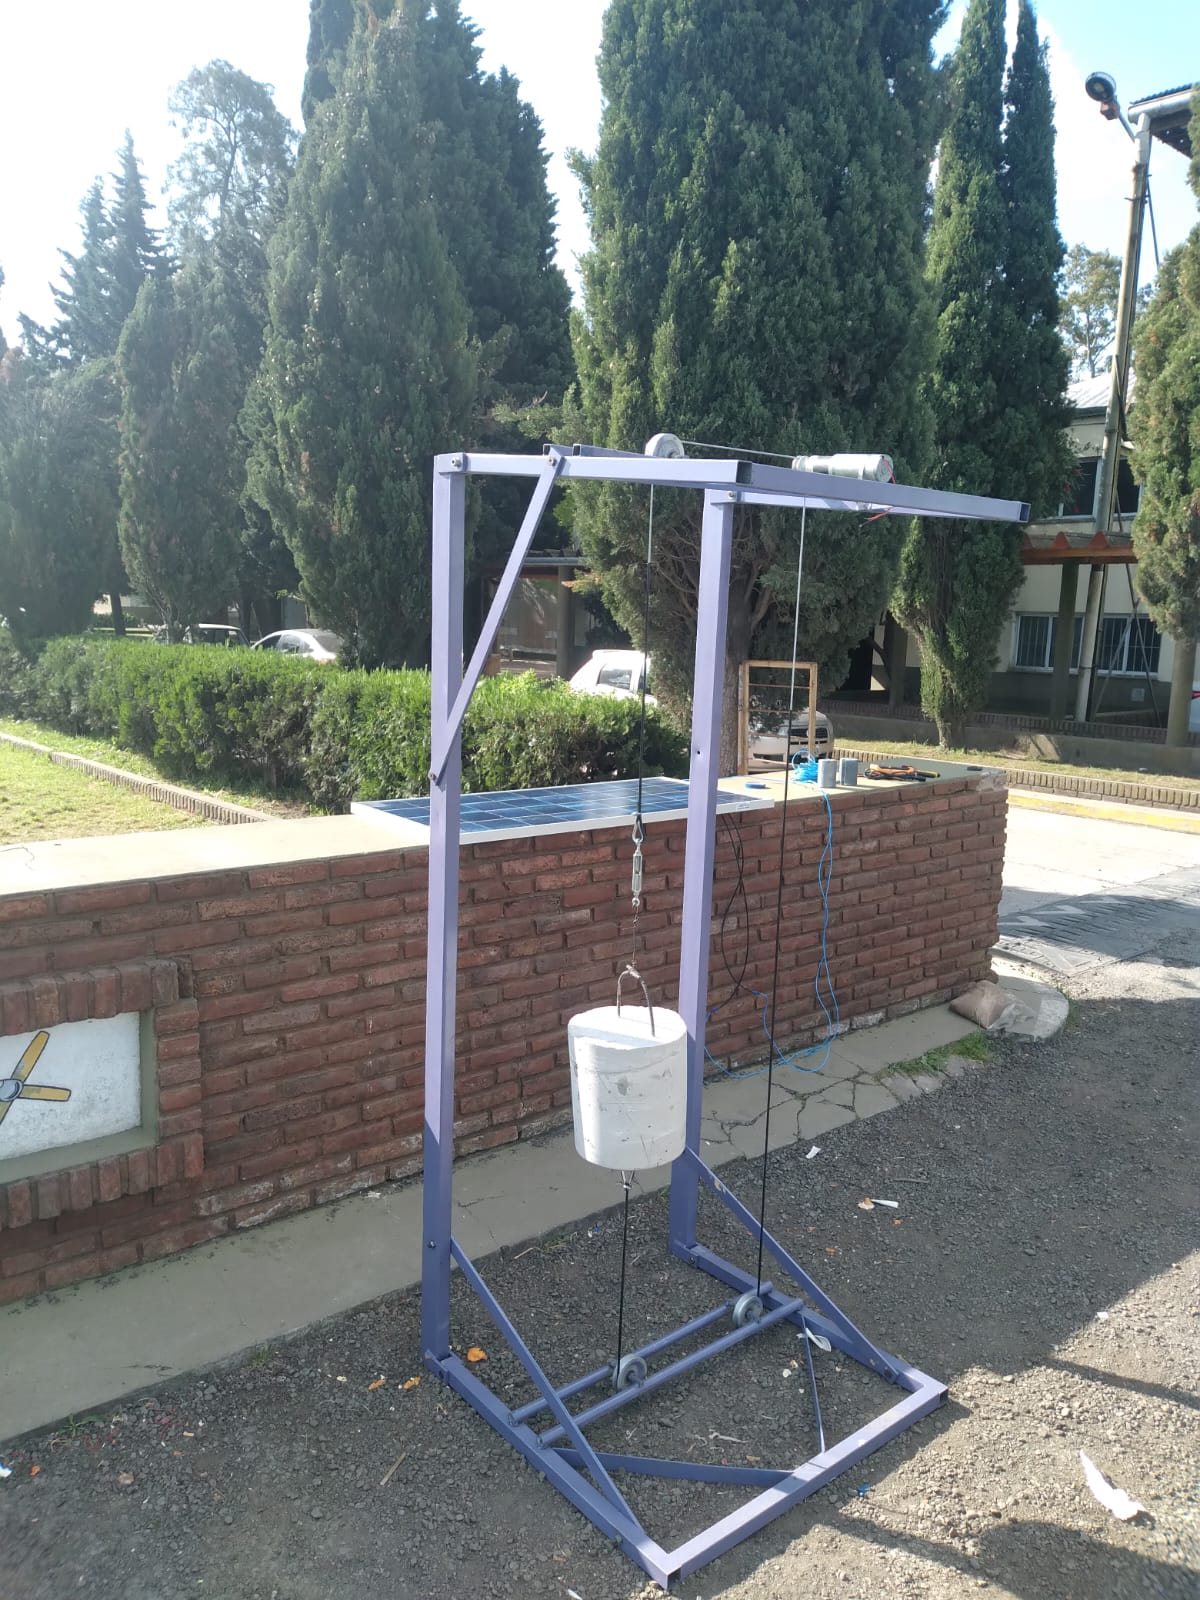
\includegraphics[width=\textwidth]{Estructura/Prototipo.png}
                    \caption{Prototipo de \textcolor{dark_violet}{\textbf{GraviCap}}}
                    \label{fig:e1.1}
                \end{subfigure}
                \begin{subfigure}[b]{0.3\textwidth}
                    \centering
                    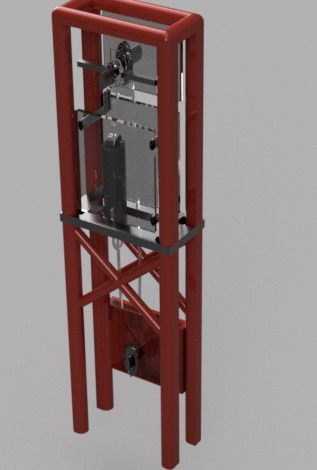
\includegraphics[width=\textwidth]{Estructura/Concepto.png}
                    \caption{Concepto de \textcolor{dark_violet}{\textbf{GraviCap}}}
                    \label{fig:e1.2}
                \end{subfigure}
                \caption{\textcolor{dark_violet}{\textbf{GraviCap}}}
                \label{fig:e1}
            \end{figure}
            
            Como alumnos, este proyecto es también una parte crucial de nuestro aprendizaje. Nos brinda la oportunidad de aplicar los conocimientos adquiridos en física, mecánica y sistemas eléctricos, además de desarrollar habilidades prácticas de diseño, ejecución y resolución de problemas. El prototipo a escala ha sido un paso esencial para comprender las implicaciones reales de implementar una batería gravitatoria, permitiéndonos abordar desafíos técnicos que probablemente también enfrentaríamos en una versión a mayor escala.\par
            El desarrollo de este prototipo nos ha proporcionado una visión clara de los beneficios y limitaciones de las baterías de gravedad, así como una base para futuras investigaciones y mejoras tecnológicas. Si bien nuestro prototipo no tiene la capacidad de almacenar grandes cantidades de energía, demuestra que esta tecnología es factible y escalable.\par
            Este enfoque educativo también nos motiva a pensar en soluciones reales para problemas energéticos actuales, como la necesidad de almacenamiento de energía renovable a gran escala, lo que refuerza la relevancia de nuestro trabajo en el contexto global de sostenibilidad y energía limpia.\par